\documentclass[a4paper,10pt]{extarticle}
\usepackage[a4paper,pdftex, margin=1in]{geometry}	% A4paper margins
\usepackage[spanish]{babel}
\usepackage[protrusion=true,expansion=true]{microtype}
\usepackage{amsmath,amsfonts,amsthm,amssymb}
\usepackage{makeidx}
\usepackage{helvet}
\usepackage{amssymb}
\usepackage{amsmath}
\usepackage{framed}
\usepackage{geometry}
\usepackage[]{graphicx}
\usepackage[utf8]{inputenc}
\usepackage{hyperref}
\usepackage{enumitem}
\usepackage{graphicx}
\usepackage[final]{pdfpages}
\graphicspath{ {images/} }
\hypersetup{
    colorlinks=true,
    linkcolor=black,
    filecolor=cyan,
    urlcolor=magenta,
}

\pagenumbering{arabic}


% --------------------------------------------------------------------
% Definitions (do not change this)
% --------------------------------------------------------------------
\newcommand{\HRule}[1]{\rule{\linewidth}{#1}} 	% Horizontal rule

\makeatletter							% Title
\def\printtitle{%
    {\centering \@title\par}}
\makeatother

\makeatletter							% Author
\def\printauthor{%
    {\centering \large \@author}}
\makeatother

\makeatletter							% Date
\def\printdate{%
    {\centering \small \@date}}
\makeatother

% --------------------------------------------------------------------
% Metadata (Change this)
% --------------------------------------------------------------------

\title{	\large \textsc{Diseño de sistemas} 	% Subtitle
		 	\\[2.0cm]								% 2cm spacing
			\HRule{0.5pt} \\						% Upper rule
			\LARGE \textbf{\uppercase{Trabajo Práctico 5:\\ Starship Game (Implementación)}}	% Title
			\HRule{0.5pt} \\ [0.5cm]		% Lower rule + 0.5cm spacing
      \vfill
      
\includegraphics[scale=0.75]{austral_logo.jpg}
}



\author{
        Perez Molina, Tomás\\[0.5cm]
}

\date{
    \today\\
}


\begin{document}

% ------------------------------------------------------------------------------
% Maketitle
% ------------------------------------------------------------------------------
\thispagestyle{empty}		% Remove page numbering on this page

\printtitle					% Print the title data as defined above
\vfill



\printauthor				% Print the author data as defined above
\printdate
\newpage
% ------------------------------------------------------------------------------
% Begin document
% ------------------------------------------------------------------------------



\tableofcontents
\thispagestyle{empty}
\pagebreak

\setcounter{page}{1} % Set page numbering to begin on this page

\pagebreak
\section{Consigna}
    \subsection{Definición}
        \paragraph{}
        Trabajando para un sitio de juegos llamado “Jug.ar” tu director de desarrollo
        decide que se debe crear un juego con naves espaciales ya que dentro de la
        amplia gama de juegos que ofrecen no hay ninguno con características. La tarea
        se delega en tu equipo y como primer paso deciden armar un prototipo de un
        juego con naves. En esta oportunidad, la tarea de llevar a cabo el diseño esta en
        tus manos.

        \paragraph{}
        Post “torbellino de ideas” (brainstorming) tu equipo y vos deciden diseñar un
        juego en el que cada jugador tenga que maniobrar su nave mientras esquiva y
        destruye meteoritos que vuelan por el espacio. Adicionalmente las naves se
        podrán destruir entre ellos y tendrán una cantidad de vidas, también serán
        destruidas por los asteroides con los que se estrellen. También deciden que al ser
        un prototipo debe ser lo mas adaptable posible por lo que concuerdan en la
        aplicación del patron MVC[1]. Para una primera versión se limitan los
        requerimientos para que el juego pueda:
        \begin{itemize}
            \item El juego sera en 2D
            \item Cada jugador podrá maniobrar su nave, a travez de una serie de teclas
            configurables (acelerar, frenar, girar). Las naves solo se pueden mover dentro
            del area correspondiente a la pantalla.
            \item Cada nave tiene la capacidad de disparar, el disparo depende del arma que
            tenga la nave, y puede disparar una o mas balas de distintos tamaños. Al
            impactar en otra nave, o en un asteroide lo destruyen y le asignan al jugador
            la cantidad de puntos correcta
            \item El escenario presenta asteroides de distintos tamaños que se mueven por la
            escena, estos aparecen desde los limites de la pantalla de forma aleatoria. (En
            principio se decide no manejar la coalición entre estos).
        \end{itemize}

        \paragraph{}
        La empresa ya dispone de algunas herramientas que se pueden usar para
        ahorrar tiempo en el diseño de este prototipo, aunque no es obligatorio:

        \paragraph{}
        La representación de un vector de dos dimensiones con sus operaciones básicas:

        \begin{center}
          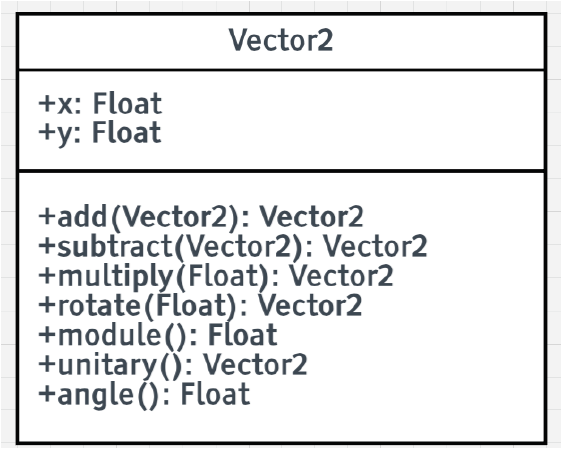
\includegraphics[scale=0.55]{vector2.png}  
        \end{center}

        \paragraph{}
        Un framework que se encarga de levantar la aplicación, el repintado constante
        de la interfaz gráfica y manejar los eventos de teclado. El método ‘draw’ se
        llama constantemente (A una frecuencia aproximada de 60 veces por segundo),
        con el finde poder actualizar el estado del juego y la interfaz gráfica. Como
        argumentos recibe tiempo que paso entre cada dibujo, así como también una
        herramienta que permite dibujar desde figuras básicas hasta el uso de imágenes,
        denominada PGraphics.

        \begin{center}
          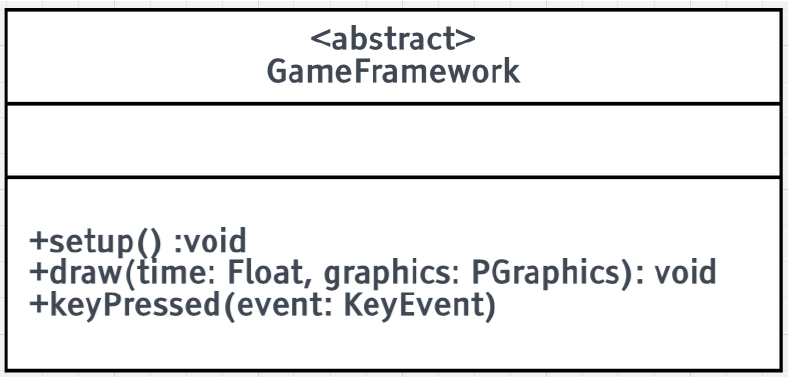
\includegraphics[scale=0.55]{game-framework.png}  
        \end{center}

        \paragraph{}
        Por ultimo existe un motor de calculo de colisiones que ya se a utilizado
        anteriormente basado la clase java.awt.Shape[2] de java.

        \begin{center}
          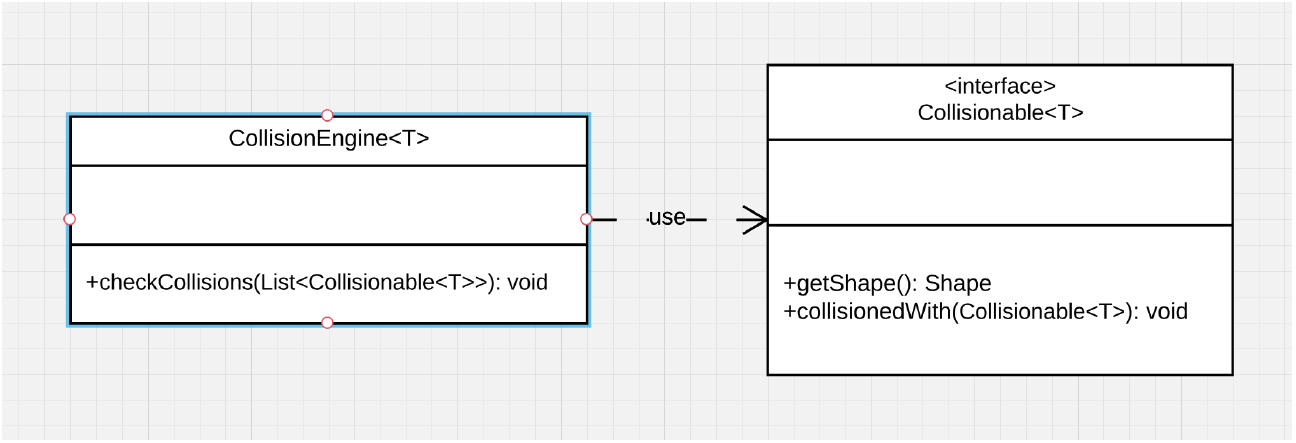
\includegraphics[scale=0.55]{collisionable.png}  
        \end{center}

        \paragraph{}
        [1] MVC = patron Model-View- Controller el cual establece que debe haber
        una clara separación entre dichas capas dentro de un sistema. El Modelo
        representara nuestro Dominio de entidades y su logica de negocio, La Vista será
        quien se encargue de mostrar los distintos estados o resultados obtenidos a partir
        del modelo y por ultimo, el Control sera quien se ocupe de orquestar la
        comunicación entre Modelo y Vista.

        \paragraph{}
        [2] https://docs.oracle.com/javase/8/docs/api/java/awt/Shape.html

    \subsection{Entrega}
        \begin{enumerate}
            \item Implementar el juego Starships a partir del diseño propuesto, realizando los cambios necesarios
            \item Modificar el UML original para reflejar los cambios realizados.
        \end{enumerate}
\pagebreak
\section{Cambios}
    \subsection{Aclaraciones}
        \paragraph{Menu}
        Los menu se limitaron a un menú principal y a un menú de pausa, lo que simplifico la interfaz para ser simplemente un \textbf{ScreenController}.

        \paragraph{Router controller}
        \textbf{BaseController} fue reemplazado por \textbf{RouterController}, que permite que las Screens tengan mas control sobre el flujo de la UI. Además ahora cada screen solo tiene un router, en vez de ser un \textbf{Observable \textless ControllerCreationObserver\textgreater}, ya que multiples routers no deberian ser notificados de los mismos cambios al mismo tiempo.

        \paragraph{Configuración}
        Se implementó \textbf{INIControlConfigurator} para configurar el juego a partir de un archivo *.ini. Que permite la definición del control de la UI, así también como la de todos los jugadores. La cantidad de jugadores siendo solo limitada por el tamaño del teclado.

        \paragraph{ProcessingKeyEventAdapter}
        Debido al manejo de KeyEvents de Processing, fue necesario incluir un \textit{adapter} que permitiera la correcta funcionalidad del KeyEventHandler propuesto en el diseño.

        \paragraph{ShipSpawner}
        Para soportar la capacidad de respawnear naves ya en juego, se agrego la interfaz \textbf{ShipSpawner} que lo permite, de esta manera se pueden dar multiple cantidad de vidas a cada jugador.

        \paragraph{Collisiones}
        Se reemplazaron los \textbf{Collision} por \textbf{Collider} que implementan la interfaz \textbf{Collisionable \textless Collider\textgreater}, de esta manera los \textbf{GameEntity} no deben implementar \textbf{Collisionable}

        \paragraph{Bounds}
        Al notar que tanto los bordes del mundo, como los de la pantalla debian ser conocidos por distintas partes de la aplicación, se implementó la clase \textbf{Bounds} para poder abstraer ese concepto y agregar alguno métodos útiles.

        \paragraph{PowerUps}
        Para permitir distintas vistas para los distintos \textbf{PowerUp}, se agrego un \textbf{PowerUpVisitor} para poder recuperar el tipo al momento de dibujar.

        \paragraph{Plane}
        Se agrego la capacidad de dibujar texto, y se cambió la interfaz de \textbf{DrawColors} para recibir un java.awt.Color

        
    \subsection{Patrones de diseño}
        \paragraph{Adapter}
        Se expandió la utilización de \textit{adapter} para poder utilizar la API de Processing con el diseño propuesto anteriormente.

        \paragraph{Visitor}
        Se agregó un \textit{visitor} de \textbf{PowerUp} para poder dibujar cada uno de diferente manera.

    \subsection{Diagramas de clases}
        \paragraph{}
        Se dividió el diagrama de clases en cuatro partes para disminuir el tamaño de los gráficos y que sea más facil la visualización.
        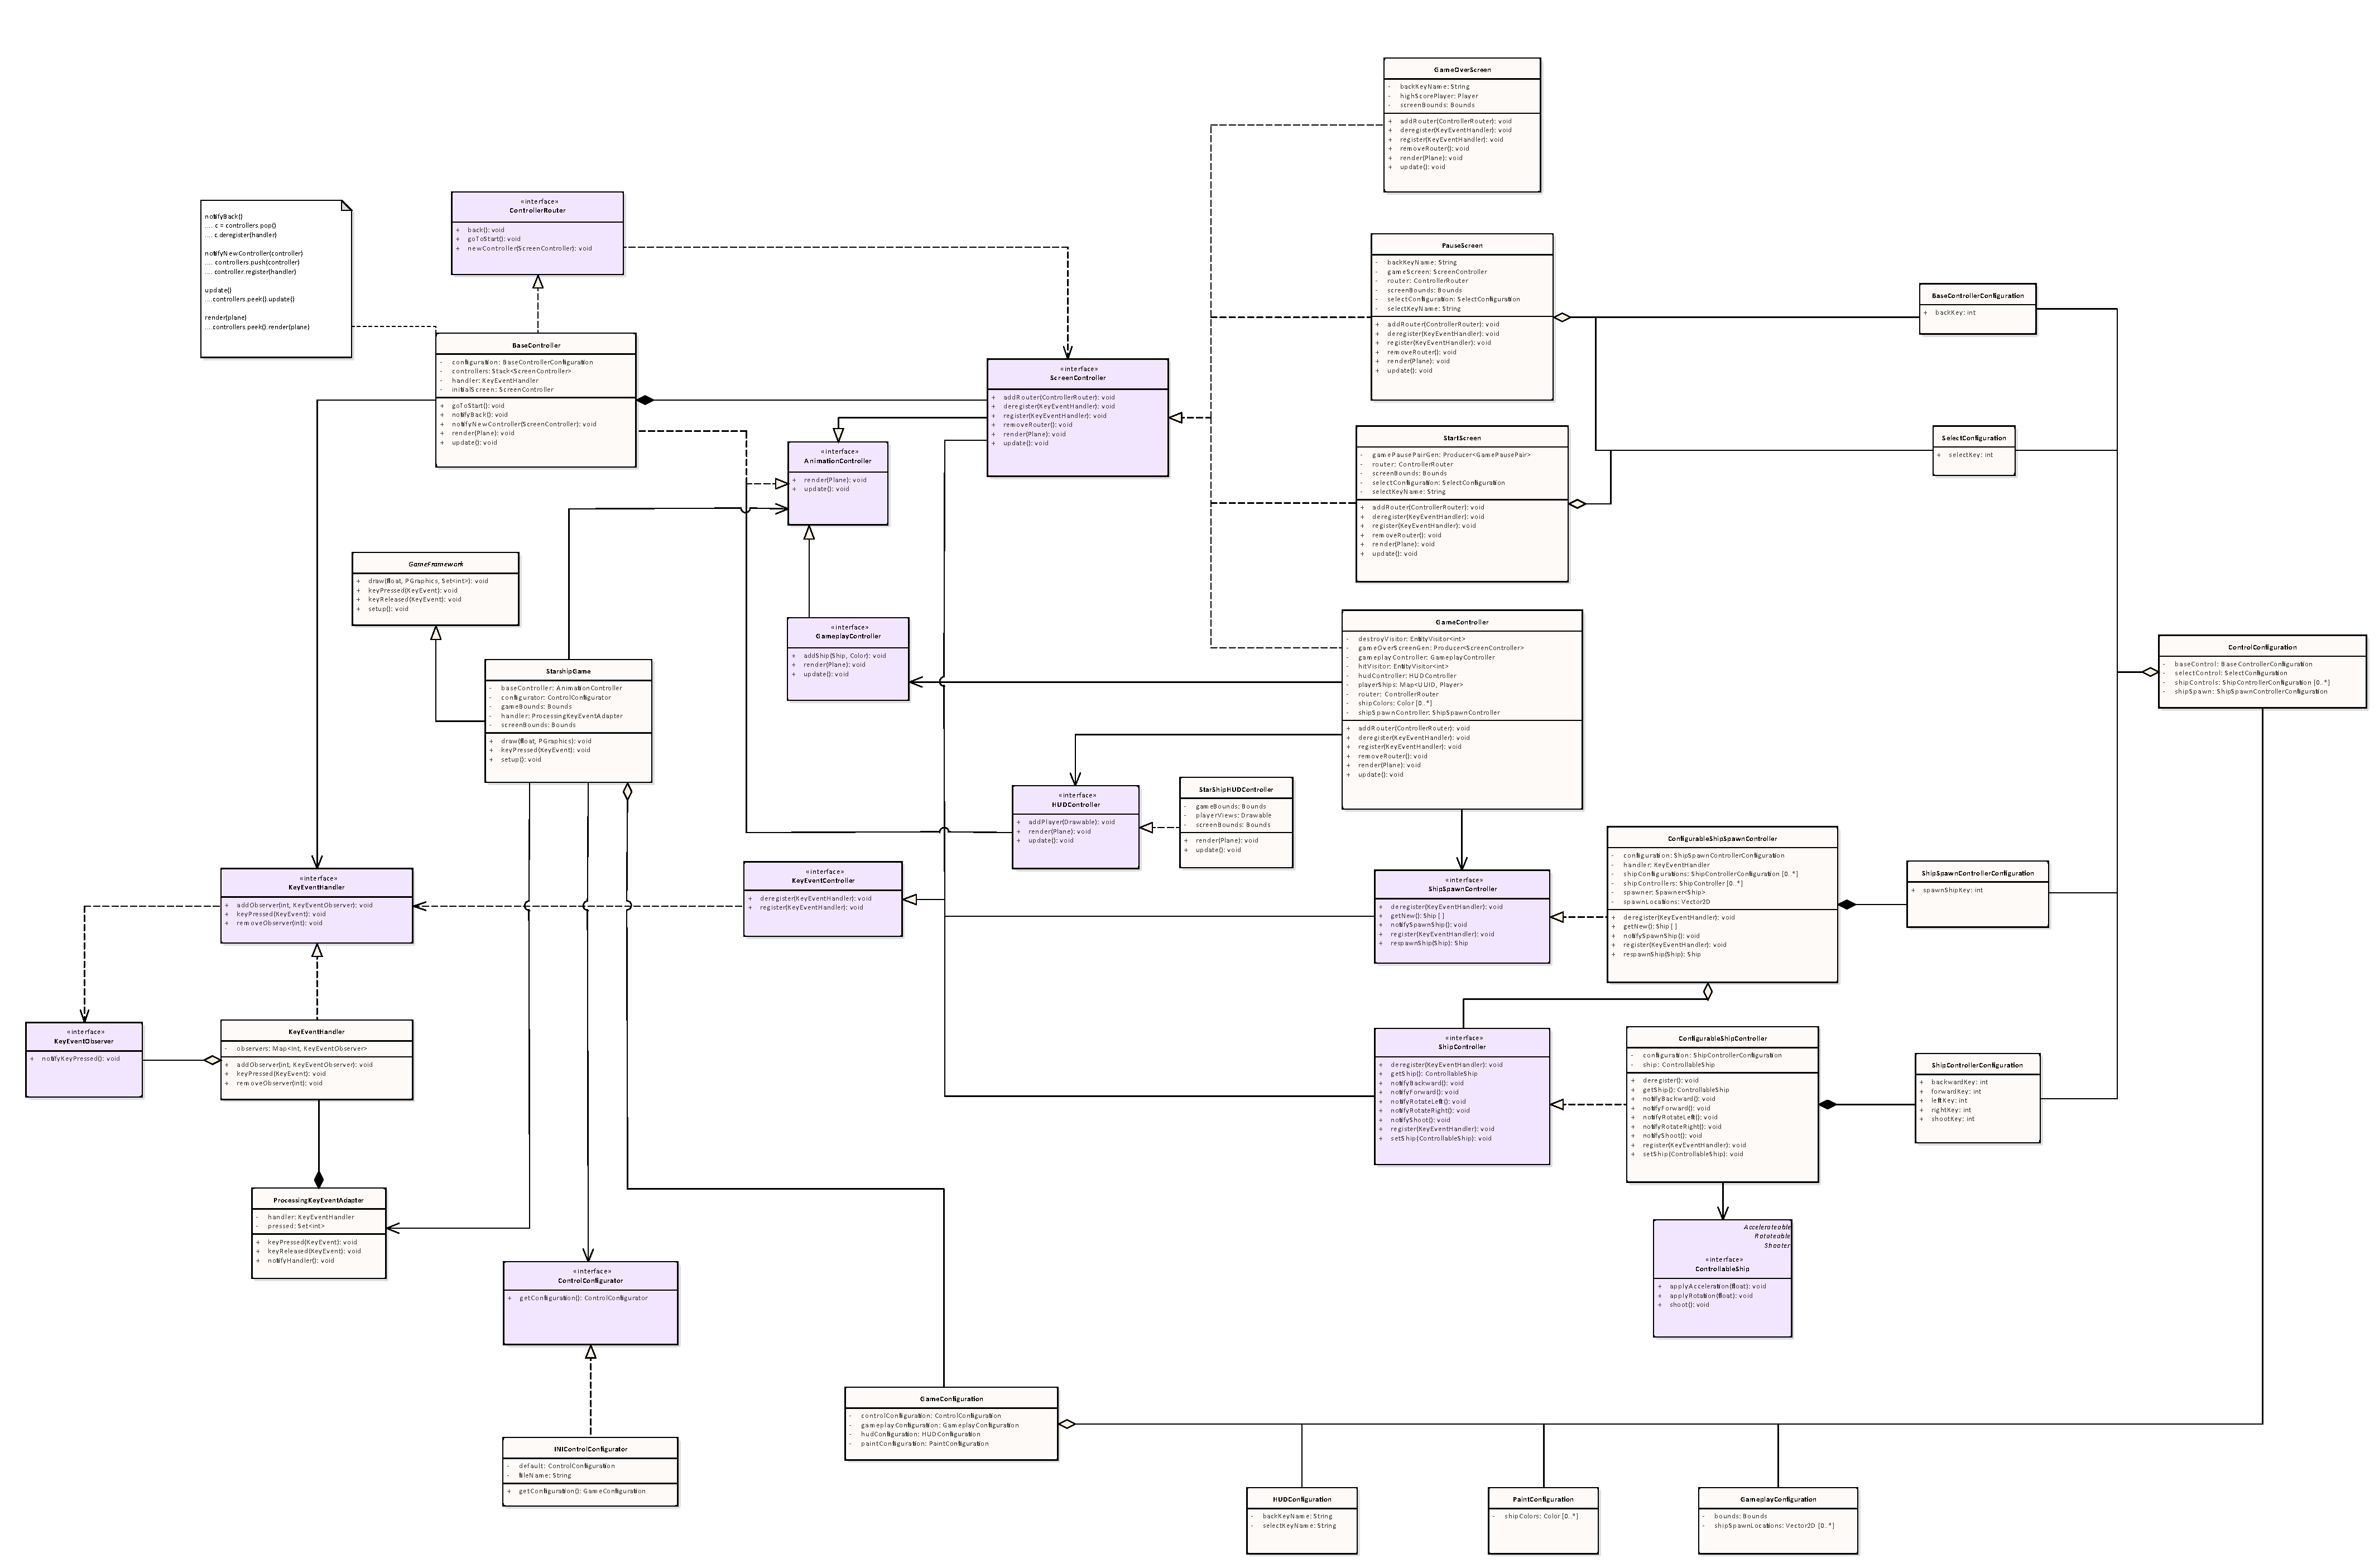
\includepdf[pages=-, fitpaper]{class-diagrams.pdf}
    
\end{document}
